\documentclass{article} 
\usepackage{amsmath,amsthm}     
\usepackage{graphicx}     
\usepackage{hyperref} 
\usepackage{url}
\usepackage{amsfonts} 
\usepackage{multicol}
\usepackage{tikz}
\usepackage{smartdiagram}
\usepackage{tabularx}
\usepackage{enumitem}
\usepackage{hyperref}
\usepackage[ruled,vlined]{algorithm2e}
\usetikzlibrary{fit}
\tikzset{
	comp/.style = {
		minimum width  = 8cm,
		minimum height = 4.5cm,
		text width     = 8cm,
		inner sep      = 0pt,
		text           = green,
		align          = center,
		font           = \Huge,
		transform shape,
		thick
	},
	monitor/.style = {draw = none, xscale = 18/16, yscale = 11/9},
	display/.style = {shading = axis, left color = black!60, right color = black},
	ut/.style      = {fill = gray}
}
\tikzset{
	computer/.pic = {
		% screen (with border)
		\node(-m) [comp, pic actions, monitor]
		{\phantom{\parbox{\linewidth}{\tikzpictext}}};
		% display (without border)
		\node[comp, pic actions, display] {\tikzpictext};
		\begin{scope}[x = (-m.east), y = (-m.north)]
			% filling the lower part
			\path[pic actions, draw = none]
			([yshift=2\pgflinewidth]-0.1,-1) -- (-0.1,-1.3) -- (-1,-1.3) --
			(-1,-2.4) -- (1,-2.4) -- (1,-1.3) -- (0.1,-1.3) --
			([yshift=2\pgflinewidth]0.1,-1);
			% filling the border of the lower part
			\path[ut]
			(-1,-2.4) rectangle (1,-1.3)
			(-0.9,-1.4) -- (-0.7,-2.3) -- (0.7,-2.3) -- (0.9,-1.4) -- cycle;
			% drawing the frame of the whole computer
			\path[pic actions, fill = none]
			(-1,1) -- (-1,-1) -- (-0.1,-1) -- (-0.1,-1.3) -- (-1,-1.3) --
			(-1,-2.4) coordinate(sw)coordinate[pos=0.5] (-b west) --
			(1,-2.4) -- (1,-1.3) coordinate[pos=0.5] (-b east) --
			(0.1,-1.3) -- (0.1,-1) -- (1,-1) -- (1,1) -- cycle;
			% node around the whole computer
			\node(-c) [fit = (sw)(-m.north east), inner sep = 0pt] {};
		\end{scope}
	}
}
\DeclareMathOperator{\diag}{diag}
\DeclareMathOperator{\E}{\mathbb{E}}
\usetikzlibrary{positioning,chains,fit,shapes,calc}
\theoremstyle{theorem}
\newtheorem{theorem}{Theorem}

\theoremstyle{definition}
\newtheorem*{definition}{Definition}
\newtheorem{assumption}{Assumption}
\newtheorem*{remark}{Remark}
\newtheorem{proposition}{Proposition}

\allowdisplaybreaks
\usepackage{collectbox}
\makeatletter
\newcommand{\mybox}{%
	\collectbox{%
		\setlength{\fboxsep}{1pt}%
		\fbox{\BOXCONTENT}%
	}%
}
\@addtoreset{footnote}{page}
\makeatother

%%%%%%%%%%%%%%%%%%%%%%%%%%%%%%%%%%%%%%%%%%%%%%%%%%
\begin{document}
	\section*{Report}
	
		\begin{tabular}{ | m{7em} | m{6.5cm}|  }  
			\hline
			Project & \textbf{Convergence guarantees for gradient descent methods on optimization for non-convex function approximation} \\
			\hline
			Student & \textbf{Hoang Trung Hieu}\\
			\hline 
			Supervisor & \textbf{Horváth Tomáš} \\
			\hline
			 Program & MSc, Applied Mathematics \\
			\hline			
			Semester & 2020/2021, Autumn \\
			\hline
		\end{tabular}
	\subsection*{Summary}
	 Federated learning (FL) is a learning paradigm seeking to address the problem of data governance and privacy by training algorithms collaboratively without exchanging the data itself. But there are some limitations: Massively distributed, non-iid dataset, the data distribution's unbalancedness. To train a neural network in general we often use the gradient decent methods to optimize the loss function. In FL, Federated Averaging(FedAvg) is used most frequently. However, it is not perfect and it performs poor-quality in some cases. My project is to analyze whether it is possible to give convergence guarantees in case the data over each devices is unbiased and evaluating of divergence between local datasets.
	
	In the first semester, my work is understanding the main concept of Federated Learning, FedAvg algorithm, and  given convergence analyses when dataset is balanced or in convex problem. Besides, I also experiment on MNIST data set and Synthetic data and illustrate by meaningful plots.	

	\subsection*{Process and Results}
	- Firstly, I took the Advanced Machine Learning Systems course \cite{cite4}, it gives a deeply analysis on the convergence of gradient decent methods. It also explains the meaning of adaptive learning rate and how it enhances the method.\\
	- These papers (\cite{cite1},\cite{cite2},\cite{cite6}) give a general look of federated learning, the challenges and limitations .\\
	- In order to attempt to analyze the convergence of FedAvg,  \cite{cite5} is a paper analysing the convergence of convex approximation function on non-iid data and \cite{cite0}  present experiments on applying different popular optimization methods for training neural networks in a federated manner. \\
	- For experiment part, the code I use from \cite{cite3} , \cite{cite31}, the dataset is MNIST and and the synthetic data is followed by \cite{cite7}. The models are 2 hidden layers neural network and 2 convolutional layers neural network.\\
		In these figures, I plot the line graphs comparing the impact of different parameters (the number of device each update(top-left), the number of epoch (top-right)batch size (bottom-left)) and impact of unbalancedness (bottom-right).
	\begin{center}
		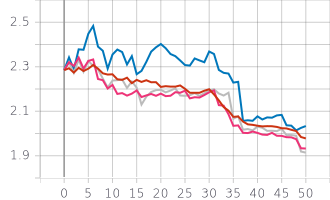
\includegraphics[scale=0.5]{Cniid.png}
		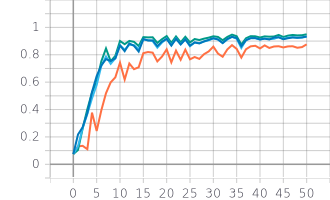
\includegraphics[scale=0.5]{E.png}
			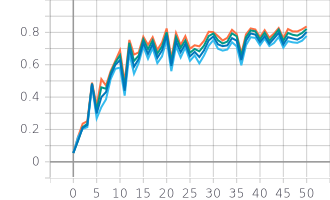
\includegraphics[scale=0.5]{B.png}	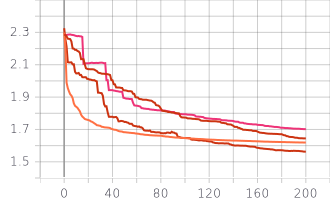
\includegraphics[scale=0.5]{syn.png}
	\end{center}	
	%\subsection*{Future work}	
	%In the next semester, I plan to develop a personalized FedAvg algorithms and evaluate this algorithm on the same data set. 	
	\begin{thebibliography}{5}
		\bibitem{cite0}
			V. Felbab, P. Kiss, and T. Horváth, (2019), \textit{Optimization in Federated Learning}, ITAT 2019
	
		
		\bibitem{cite1}
		F. Sattler, S. Wiedemann, K. Müller, W. Samek,  (2019), \textit{Robust and communication-efficient federated learning from non-iid data},IEEE transactions on neural networks and learning systems,
		\bibitem{cite2}
		H. Brendan McMahan, Eider Moore, Daniel Ramage, (2017) , \textit{Communication-Efficient Learning of Deep Networks
			from Decentralized Data}, \href{https://arxiv.org/abs/1602.05629}{https://arxiv.org/abs/1602.05629}  
		\bibitem{cite3}
		\textit{TensorFlow Federated}, \href{ https://github.com/tensorflow/federated }{https://github.com/tensorflow/federated}
			\bibitem{cite31}
		\textit{On the Convergence of FedAvg on Non-IID Data
			repository}, \href{ https://github.com/lx10077/fedavgpy }{https://github.com/lx10077/fedavgpy}
		\bibitem{cite4}
	\textit{Advanced Machine Learning Systems Course} , (2017),  \href{https://www.cs.cornell.edu/courses/cs6787/2017fa/}{https://www.cs.cornell.edu/courses/cs6787/2017fa/}	
		\bibitem{cite5}
		X. Li, K. Huang, W. Yang, S. Wang, Z. Zhang, (2019),  \textit{On the Convergence of FedAvg on Non-IID Data}, \href{https://arxiv.org/abs/1907.02189}{https://arxiv.org/abs/1907.02189}
		\bibitem{cite6}
	J. Konečný, H. B. McMahan, D. Ramage, P. Richtárik, (2016),  \textit{	Federated Optimization Distributed Machine Learning for On-Device Intelligence} \href{https://arxiv.org/abs/1610.02527}{https://arxiv.org/abs/1610.02527}
	\bibitem{cite7}
		A. K. Sahu, T. Li, M. Sanjabi, M. Zaheer, A. Talwalkar, and V. Smith, (2018), 
		\textit{Federated optimization for heterogeneous networks}, \href{https://arxiv.org/abs/1812.06127}{https://arxiv.org/abs/1812.06127}
	\end{thebibliography}
\end{document}